\documentclass[conference]{IEEEtran}

\ifCLASSINFOpdf
  % \usepackage[pdftex]{graphicx}
  % declare the path(s) where your graphic files are
  % \graphicspath{{../pdf/}{../jpeg/}}
  % and their extensions so you won't have to specify these with
  % every instance of \includegraphics
  % \DeclareGraphicsExtensions{.pdf,.jpeg,.png}
\else
  % or other class option (dvipsone, dvipdf, if not using dvips). graphicx
  % will default to the driver specified in the system graphics.cfg if no
  % driver is specified.
  % \usepackage[dvips]{graphicx}
  % declare the path(s) where your graphic files are
  % \graphicspath{{../eps/}}
  % and their extensions so you won't have to specify these with
  % every instance of \includegraphics
  % \DeclareGraphicsExtensions{.eps}
\fi


\usepackage{graphics}
\usepackage{lmodern}
\usepackage{epstopdf}
\usepackage{biblatex} 
\bibliography{report_giorgos} 

% correct bad hyphenation here
\hyphenation{op-tical net-works semi-conduc-tor}


\begin{document}

%
% paper title
% can use linebreaks \\ within to get better formatting as desired
\title{Bare Demo of IEEEtran.cls for Conferences}


% author names and affiliations
% use a multiple column layout for up to three different
% affiliations
\author{\IEEEauthorblockN{Michael Shell}
\IEEEauthorblockA{School of Electrical and\\Computer Engineering\\
Georgia Institute of Technology\\
Atlanta, Georgia 30332--0250\\
Email: http://www.michaelshell.org/contact.html}
\and
\IEEEauthorblockN{Homer Simpson}
\IEEEauthorblockA{Twentieth Century Fox\\
Springfield, USA\\
Email: homer@thesimpsons.com}
\and
\IEEEauthorblockN{James Kirk\\ and Montgomery Scott}
\IEEEauthorblockA{Starfleet Academy\\
San Francisco, California 96678-2391\\
Telephone: (800) 555--1212\\
Fax: (888) 555--1212}}

% conference papers do not typically use \thanks and this command
% is locked out in conference mode. If really needed, such as for
% the acknowledgment of grants, issue a \IEEEoverridecommandlockouts
% after \documentclass

% for over three affiliations, or if they all won't fit within the width
% of the page, use this alternative format:
% 
%\author{\IEEEauthorblockN{Michael Shell\IEEEauthorrefmark{1},
%Homer Simpson\IEEEauthorrefmark{2},
%James Kirk\IEEEauthorrefmark{3}, 
%Montgomery Scott\IEEEauthorrefmark{3} and
%Eldon Tyrell\IEEEauthorrefmark{4}}
%\IEEEauthorblockA{\IEEEauthorrefmark{1}School of Electrical and Computer Engineering\\
%Georgia Institute of Technology,
%Atlanta, Georgia 30332--0250\\ Email: see http://www.michaelshell.org/contact.html}
%\IEEEauthorblockA{\IEEEauthorrefmark{2}Twentieth Century Fox, Springfield, USA\\
%Email: homer@thesimpsons.com}
%\IEEEauthorblockA{\IEEEauthorrefmark{3}Starfleet Academy, San Francisco, California 96678-2391\\
%Telephone: (800) 555--1212, Fax: (888) 555--1212}
%\IEEEauthorblockA{\IEEEauthorrefmark{4}Tyrell Inc., 123 Replicant Street, Los Angeles, California 90210--4321}}




% use for special paper notices
%\IEEEspecialpapernotice{(Invited Paper)}




% make the title area
% IEEEtran.cls defaults to using nonbold math in the Abstract.
% This preserves the distinction between vectors and scalars. However,
% if the conference you are submitting to favors bold math in the abstract,
% then you can use LaTeX's standard command \boldmath at the very start
% of the abstract to achieve this. Many IEEE journals/conferences frown on
% math in the abstract anyway.

% no keywords




% For peer review papers, you can put extra information on the cover
% page as needed:
% \ifCLASSOPTIONpeerreview
% \begin{center} \bfseries EDICS Category: 3-BBND \end{center}
% \fi
%
% For peerreview papers, this IEEEtran command inserts a page break and
% creates the second title. It will be ignored for other modes.
\IEEEpeerreviewmaketitle



\section{Learning}
Learning and planning in this setting is not trivial and can only be achieved through several techniques that allow us to represent the huge state and action space of the \textit{Domination Game} in a minimalistic way. First of all, we are dealing with a continuous state space in respect to the agents' positions, the observations about our opponent agents, the amount of ammo that we have - can be an integer from zero to infinite theoretically, and the general statistics about the game which could be represented by a huge number of discrete integer values. As an example, we can represent the score of the game as a really informative feature of our state space. However, to represent the score you need all 2-decimal point float numbers between $0.00$ and $1.00$, which are $101$ discrete states. In this case, techniques like keeping only the first decimal point of the score value leads to a huge decrease in the number of states, i.e. 11 states. Hence the state space of this game grows rapidly in respect to the number of features we use to represent the state and the action space of our agents. As it is referred in~\cite{boutilier2011decision}, the biggest difficulty when we are dealing with state-based problem formulations, is the \textit{curse of dimensionality}, the state action space grows exponentially with the number of features. We can see this \textit{Domination Game} problem as a \textit{Markov Decision Process}, which is fully observable in respect to our agents' positions, the control points' state, and the game state. However, we have partial observability for the opponent agents, which of course can be represented as full observable case only when opponents are in our field of view.

\subsection{Grid World}
In this subsection, we formalize the problem, and we define the state and action state space, that we used in the first and most simple approach.
\subsubsection{State-Action Space}
Our first approach to deal with the problem of the continuous state space was to split the map into tiles of size $16\times16$, which was also the original tile size of the game itself. A method which is similar with \textit{tile coding}, as it is described in Chapter~$7$ of \emph{Hado Van Hasselt} book, about \textit{Continuous State and Action Spaces}. So, the first feature of our state space is the position of our agent in this grid world, meaning the closest from our agent tile coordinate in the 2D space, given by the \textit{Euclidean distance}. For example, the states of the agent position can be given by, 
\begin{equation}
S_{position} = \lbrace (0,0),\ldots,(World_{width} / 16, World_{height} / 16)  \rbrace
\end{equation} 
The second feature of the state space is the \textit{Control Points State}, each control point can be the following states,
\begin{equation}
S_{cps} = \lbrace -1, 0, 1 \rbrace
\end{equation}
$-1$, when is dominated by the opponent team, $0$, when is neutral, and $1$ when is occupied y our team. Given that we have two control points in our map the state that is able to describe the \textit{Cps} state space is the following, 
\begin{equation}
S_{full\_cps} = S_{cps} \times S_{cps} 
\end{equation}
, which is the cross product between the two control points' states. 

For the action space, each agent had all neighboring tiles to drive there or to stay in the same position, resulting to 9 actions for each given tile. However, actions which would lead the agent hit a wall in the map excluded from selection. So the final state space will be:
\begin{equation}
S = S_{position} \times S_{full\_cps} \times A
\end{equation}
\subsubsection{Reward Function}
The reward function in this approach was obtained by a single function, which was checking the difference between the previous and the current condition of the \textit{Cps} state.
\begin{equation}
Reward = (S^{t}_{full\_cps(i)} - S^{t-1}_{full\_cps(i)}) \times 10, \forall i \in \lbrace 0,1 \rbrace
\end{equation}
\begin{equation}
Reward = Reward + (Ammo^{t} - Ammo^{t-1}) \times 4
\end{equation}
There was also a reward when the agent succeed to obtain ammo, but weighted less that the reward for capturing a control point.

\subsubsection{Learning Method}
We decided, to implement \textit{independent Q-Learning} for each one of our agents. Each agent holds its own \textit{Q-table}. The states that an agent can be are the possible position in the grid world, together with the state of the control points. Furthermore, in each of these states, it has a set of possible action that can lead the agent to drive in a neighboring tile. The update rule of the \textit{Q-Learning}, was updating the table of each independent agent every time the agent reached its target location, i.e. its previous action. We used \textit{Q-Learning} with $0.7$ learning rate-$\alpha$ and the same value for discount factor-$\gamma$.

\subsubsection{Results}
The results of this approach was tested in two settings. The first setting was on the same map but on a \emph{1vs1} game. The second approach, was the original game \emph{3vs3}. The results of \textit{independent Q-Learning} in this grid world representation of the problem were really bad and we think that are not even worth to be mentioned here. One explanation is that we have no information in the state space referring to the agent's orientation. So, each agent can easily choose target locations that are located in its backward direction and this caused the agents to perform really slow turns and causing a delay to the completion of their actions, as well as the update rule for several game steps.

\subsection{Interesting Points as States}
In the previous subsection, we described an easy way to formalize the problem of learning in this Markov decision process setting. Our approach for selecting an ideal state and action space was not really applicable to this game. In this subsection, we are presenting a better way to represent the state and the action space.
\subsubsection{State-Action Space}
In \textit{Domination Game}, there are four important points in the map, the two control points and the two ammo spots. Furthermore, the initial positions of the agents can be described as an important point as well. Here, we are investigating the use of these important spots into the map as states in the MPD representation of our learning problem. Hence the feature describing the position is an important point of the map. This can be described as:
\begin{equation}
S_{position} = \lbrace CP_1, CP_2, AM_1, AM_2, INIT  \rbrace
\end{equation}
But, this is a really tiny representation in contrast to the previous one, which had a grid over all map positions. So, we decided to represent a joint state space which includes information for all the three agents. Agents now, will decide their action not only depending on their own locations, but also on where their teammates are located.
\begin{equation}
S'_{position} = S_{position} \times S_{position} \times S_{position}
\end{equation}
The first position in this product is always referring to the agent who updates its \textit{Q-table}, and the other two positions are referring to the other two agents in lexicographic order.

The current position state of each agent is given always by its previous visited state in this state space and the action is represented by the driving goal of the agent. We also used the state of the control points as they were described in equation (3). Third component of our state space is the opponents' positions. However, our agents are not always aware of the opponents' positions in the map, due to the limited range they can observe. As a result, we decided to represent our knowledge about the opponents as a vector of four elements, as many as the interesting points in the map except from our initial position. Each element in this vector can take integer values from $0$ to $3$, representing how many opponent agents are located near to each state.
\begin{equation}
S_{foes} = \lbrace <0,0,0,0>, <0,0,0,1>, \ldots, <0,0,0,3>  \rbrace
\end{equation}
The knowledge of the opponents' positions is known to all of our agents, even only one agent from our team can see opponents.

For the action space, each agent had all possible position states except from the initial position.
The action set was:
\begin{equation}
A = \lbrace CP_1, CP_2, AM_1, AM_2 \rbrace
\end{equation}
The state-action space is now:
\begin{equation}
S = S'_{position} \times S_{full\_cps} \times S_{foes} \times A
\end{equation}
Comparing with the previous approach described in the above subsection, we can realize that this one is more compact and it allow to us use more information.
\subsubsection{Reward Function}
The reward function is the same as described in the grid world approach.
\subsubsection{Learning Method}
One more time, we decided, to implement \textit{independent Q-Learning} for each one of our agents. Now, each agent does not hold its own \textit{Q-table}, but all agents update the same table. We can see it as a group of agents try to learn a symmetric optimal policy. As an example, imagine there are two agents in states A,B respectively. The optimal action for agent one, in state A and agent two in state B, is the same as the optimal action for the second agent in state A and agent one in state B. Again, the update rule of the \textit{Q-Learning}, updates the table of each independent agent every time the agent reaches its target state, i.e. its previous action. We used \textit{Q-Learning} with $0.7$ learning rate-$\alpha$ and the same value for discount factor-$\gamma$.
\subsubsection{Results}


\subsection{Interesting Points and Transitions as States}
We saw, how the performance of our agent improved using interesting points as the state space of our MDP framework. Here, we are investigating one more improvement that can lead us to a better learning scheme.In general, considering only interesting points as states, causes really delays at the update rule of \textit{Q-learning} for example. Furthermore, there might be also a lot of changes in the world state while an agent is in a transition from its previous state to another. Imagine for example, that agent A chooses an action towards the control point 1. Simultaneously, agent B chooses the same action, agent A reaches control point 1 first, but agent B cannot change its action and is forced to go to the control point no matter if it is taken by its teammate. Thus, there is a need of additional states which are going to describe transitions from one state to another. This idea is exploited through the next parts of this paper, as our last and best hope to acquire a better performance for the agent.
\subsubsection{State-Action Space}
As in previous part in this section, we are going to describe each part of the MDP representation. First of all, the feature of the state space which is going to represent the position of each agent is now different. Given a set of states as in eq. (7), and a set of transitions T, the new state space will be:
\begin{equation}
S_{position} = \lbrace CP_1, CP_2, AM_1, AM_2, INIT  \rbrace
\end{equation}
\begin{equation}
T_{position} = permutations(S_{position}, S_{position})
\end{equation}
\begin{equation}
S'_{position} = chain(S_{position}, T_{position})
\end{equation}
So, the agent now, can be in state:
\begin{itemize}
\item I am in state $CP_1$ or,
\item I am going from $CP_1$ to $CP_2$.
\end{itemize}
As you can realize, this is a simple way to add more information about states. Unfortunately, this is the state space now is impossible to contain the same amount of information about the teammates of our agent. So, we decided, in order to keep it feasible computationally, to represent the state of our teammates with their goal, again, in lexicographical order.
\begin{equation}
S''_{position} = S'_{position} \times S_{position} \times S_{position} 
\end{equation}
In this test case, we are not using the information for the opponent agents' positions, in order to keep it computationally tractable, but we use the Cps states from eq. (3).

\begin{figure}
    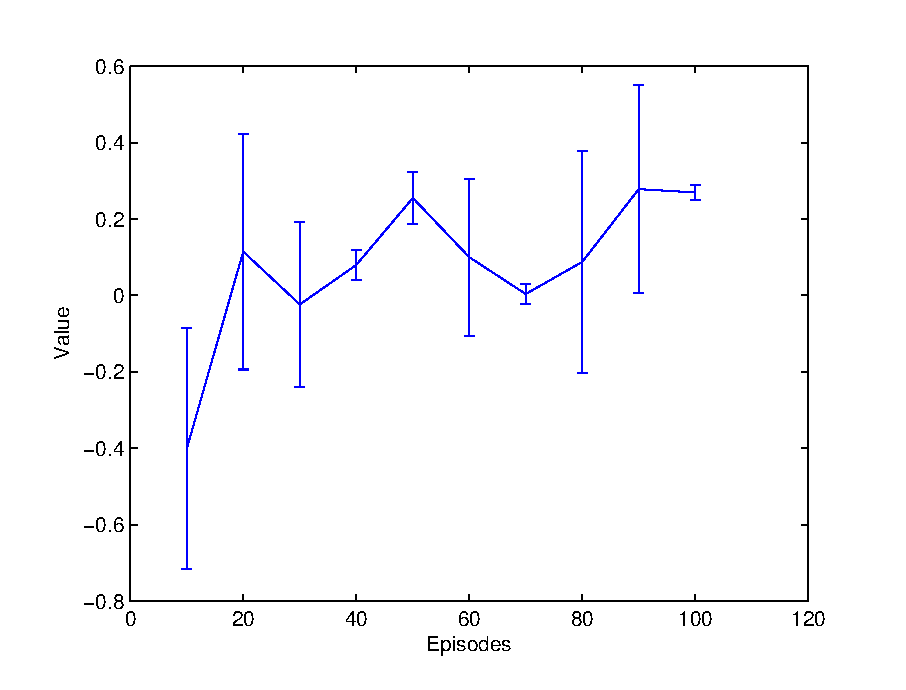
\includegraphics[width=0.4\textwidth]{figures/snake1vs1.eps}
\end{figure}

For the action space, each agent has all possible position states except from the initial position.
The action set is the same as before.
\begin{equation}
A = \lbrace CP_1, CP_2, AM_1, AM_2 \rbrace
\end{equation}
The state-action space is now:
\begin{equation}
S = S''_{position} \times S_{full\_cps} \times A
\end{equation}
\subsubsection{Reward Function}
The reward function is the same as described in the grid world approach. This function is described in eq. (5-6).
\subsubsection{Learning Method}
The reason why we chose to implement \textit{Independent Q-Learning} not only in this test case, but in the previous test cases as well, was the fact that the state-action space then was really intractable. Almost $500Mb$ was the value table when we tried to include joint actions in our state and action space, which is indicative about how much the state space grows in a multi-agent setting.
Again, the update rule of the \textit{Q-Learning}, updates the table of each independent agent every time the agent reaches its target state, i.e. its previous action. We used \textit{Q-Learning} with $0.7$ learning rate-$\alpha$ and the same value for discount factor-$\gamma$. Each update rule is performed after each game-step and not like the previous case, when the update rule was only performed after each arrival in the target state.
\subsubsection{Results}


\subsection{}

\newpage
\printbibliography 

% that's all folks
\end{document}


